\documentclass[main.tex]{subfiles}
\setlength{\columnsep}{3cm}
\begin{document}

\addtolength{\tabcolsep}{-2pt}

\section{Thread Communication}
Now that we discussed what a thread is and how parallelism and concurrency are achieved at the OS level, we are ready to talk about how to organize parallelism.\\
In this section we take for granted that we have a Java program with multiple threads running \textit{concurrently} and discuss issues that arise and how to solve them when programming in this manner.

\subsection{A Simple Multi-Threaded Program: Interleavings}
Let us now write our first multi-threaded Java program. We want to write a method that takes two int arrays as an argument, sorts them and then prints the smallest elements of both arrays to the console. Since we know how to create a thread in Java, this is a simple task:
\begin{minted}[]{java}
public void printSmallest(int[] a, int[] b) {
    /* We first create a Thread object sorting the first array.
    * Then, the main thread sorts the second array and prints to the console. */
    Thread t = new Thread() {
        public void run() {
            // This code is executed when the thread is started.
            Arrays.sort(a);
        }
      };
    t.start();
    Arrays.sort(b);
    System.out.println(a[0] + " " + b[0]);
}
\end{minted}
We might expect the method to print the smallest element of both arrays. However, when running the program multiple times, we see that this is not always the case. This is because the main thread and the created thread are running concurrently. As soon as t is started, we have two threads running concurrently, which we can imagine as two [sequential] Java programs running at the same time:
\begin{figure}[H]
    \begin{subfigure}[t]{.6\textwidth}
        \texttt{Main Thread}:
        \begin{minted}[]{java}
Arrays.sort(a);
System.out.println(a[0] + " " + b[0]);
        \end{minted}
    \end{subfigure}%
    \begin{subfigure}[t]{.6\textwidth}
        \texttt{Helper Thread t}:
        \begin{minted}[]{java}
Arrays.sort(b);
        \end{minted}
    \end{subfigure}
\end{figure}
It can occur that the main thread executes the println statement before the created thread can sort the array a. This now all depends on how the OS schedules these threads.\\
We call the (actual real-time) order that instructions of multiple threads are executed in \textbf{interleavings}. In this case, there are interleavings where the main thread prints before the other thread finishes sorting the array. Since this is not what the program is intended to do, we call this a \textit{bad interleaving}. \\[3mm]
Note that interleavings do not necessarily refer to the interleaving of Java instructions, but rather the interleaving of the machine instructions that are compiled from the Java code.\\
We will soon discuss solutions to the problem (which is waiting for the helper thread to finish in this case) and other approaches to control the execution of our Java threads. But first, we have to talk about thread states in Java.

\subsection{Thread States [2]}
Even though we said in the previous chapter that Java threads are 1-to-1 mapped to OS threads, we can still control our Java threads from within our program. The Java Thread library exposes many tools for managing running threads to the programmer. For example do we have various methods that cause a thread not to be scheduled by the OS. To be able to talk about the effects of different thread operations, we need some notion of \textit{thread states}. A Java thread typically goes through the following states:
\begin{itemize}
    \item \textit{New}: Once the Thread object is created, the thread enters the new state. At this point, the thread is just an object in the heap and no resources have been allocated for it.
    \item \textit{Runnable}: Once we call \textbf{start()} on the new thread object, the system allocates resources to enable its execution and the thread becomes eligible for being scheduled.
    \item \textit{Running}: When the thread is actually scheduled to run.
    \item \textit{Not runnable}: We use this as an umbrella state for multiple states that cause the thread to not be runnable. The thread enters this state when one of the following events occur:
        \begin{enumerate}
            \item The sleep() method is called to suspend the thread for a specified amount of time to yield control to the other threads.
            \item The wait() method is called to wait for a specific condition to be satisfied.
            \item The thread is blocked and waiting for an I/O operation to be completed. Attempting to acquire a lock and calling join() will also cause a thread to be blocked, but these two topics will be covered later on.
        \end{enumerate}
    These methods and terms will be covered in this chapter. At this point we just note that even though our Java threads are scheduled by the OS, we still have \textit{some} control over them from the language itself.
    \item \textit{Terminated}: A thread transitions to terminated state when the run() method terminates and exits.
\end{itemize}
\begin{figure}[H]
    \centering
    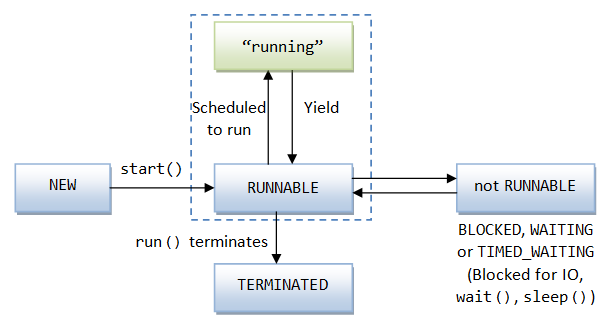
\includegraphics[scale=0.8]{ThreadLifeCycle.png}
    \caption{Java Thread States: https://www3.ntu.edu.sg/home/ehchua/programming/java/j5e\_multithreading.html}
\end{figure}
There is a getState() method in Java returning one of the states \textit{new}, \textit{runnable}, \textit{blocked}, \textit{waiting}, \textit{timed waiting} and \textit{terminated}:
\begin{minted}[]{java}
Thread t = new Thread() {
    public void run() {
        System.out.println(Thread.currentThread().getState());
    }
  };
t.start();

> RUNNABLE // prints the state to the console
\end{minted}
We notice that Java differentiates some states we simply put into a \textit{not runnable} state. These roughly correspond to the three reasons we mentioned for entering a not runnable state. We need to introduce a few more topics before we can differentiate these properly. For the moment, just appreciate that we have the power of putting our running Java Thread objects into a certain state resulting in the underlying OS thread not getting scheduled.

\subsection{Waiting for Another Thread}
\subsubsection{Busy Waiting}
Consider the program from 1.1 again. Our issue was that the main thread did not wait until the other thread completed. A solution to this is to check in a while-loop if the other thread already terminated. With our new knowledge about Java thread states, we can check the state of Thread t using the getState() method. When the while condition fails, we can finally print:
\begin{minted}[]{java}
public void printSmallest(int[] a, int[] b) {
    Thread t = new Thread() {
        public void run() {
            Arrays.sort(a);
        }
      };
    t.start();
    Arrays.sort(b);
    while(t.getState() != Thread.State.TERMINATED) {
        // wait for t to terminate
        System.out.println("Waiting...");
    }
    System.out.println(a[0] + " " + b[0]);
}

> Waiting... // example output of this program to the console
  Waiting...
  Waiting...
  Waiting...
  1 1 // 1 is the smallest element of both arrays.
\end{minted}
This program is expected to work in \textit{most} cases. However, there are two things wrong with it:
\begin{itemize}
  \item The first concerns the getState() method. We introduced thread states in the previous section and checking such a condition makes sense at first. However, the Java documentation itself states that the method is designed for \textit{monitoring the system state} and not for concurrency control.\\
  This means that Java does not guarantee that the returned state is correct and hence we consider the program to not be correct. %We have to be careful with methods that rely on a notion that is provided by Java (like the Java thread states), since the threads are primarily controlled by the OS.
  \item While the helper thread is still running, the main thread keeps checking its state in a while loop. This is referred to as \textit{busy waiting}. The thread is not performing meaningful work. However, the OS does not know this and will still schedule this thread, using up CPU time. Ideally, we would tell the OS that it should not schedule the main thread as long as the other thread is running. This is achieved by the join() method introduced in the next section.
\end{itemize}
\subsubsection{join()}
The join() method does exactly what we were looking for in our example program. When we call t.join() in the example, the main thread (which is the one executing the statement) pauses its execution until t terminates. We can replace the while loop with a call to t.join().
\begin{minted}[]{java}
public void printSmallest(int[] a, int[] b) {
    Thread t = new Thread() {
        public void run() {
            Arrays.sort(a);
        }
      };
    t.start();
    Arrays.sort(b);
    try {
        t.join();
    } catch (InterruptedException e) {
        e.printStackTrace();
    }
    System.out.println(a[0] + " " + b[0]);
}
\end{minted}
The program now works as expected and there are no bad interleavings possible anymore. Note that calls to join() have to be put into a try-catch block because join() can throw an InterruptedException, which we need to handle.\\[3mm]
Now think about what would happen if the main thread would first call t.join() and only then sort the array:
\begin{minted}[]{java}
t.start();
t.join(); // in real code, this should be in a try-catch block
Arrays.sort(b)
\end{minted}
\textbf{Solution}: This code still works, but it is slower. This is because as soon as the main thread calls t.join() it will not be scheduled anymore until t terminates. Only then will it sort the array 'b'. This means that first, array 'a' is sorted and then array 'b', which is no improvement over sequential code.

\subsubsection{Busy Waiting vs Joining}
We mentioned the drawbacks of busy waiting (waiting thread gets scheduled, taking away CPU time). However, joining is not always better. Calling join() can result in a context switch: The thread will be descheduled and some other thread will be scheduled in its stead (maybe the helper thread - but maybe a different one altogether).\\
When this context switch takes more time than the work of the joined thread, we would have been better off just busy waiting. So, for a very short-lived thread, it may be more efficient to simply busy wait than to call join(). However, in almost all cases, calling join() will be better.

\subsection{Interrupting a thread}
% \subsubsection{Interrupting a running thread}
\subsubsection{interrupt() on a Runnable Thread}
Assume that t is a Java Thread object in the following.\\
When we want to prematurely stop t, we can do so by calling t.interrupt():
\begin{minted}[]{java}
public void interruptThread() {
    Thread t = new Thread() {
        public void run() {
            work() // Thread performs some work
            System.out.println("Finished!");
        }
    };
    t.start();
    t.interrupt(); // interrupt the thread
}

> Finished! // console output
\end{minted}
When we run this program, nothing seems to happen. Even though t is interrupted, it finishes its work and prints happily to the console.\\
This is because interruption in Java is implemented with a flag (a flag is just a boolean value). We can imagine that each Thread object in Java has a boolean attribute called 'interrupted'. A thread can set the flag of another by calling interrupt() on it. The interrupted Thread object can decide itself what happens upon having its flag set.\\
The isInterrupted() method returns whether the current thread has its interrupted flag set. Let us check in the t.run() method if t is interrupted:
\begin{minted}[]{java}
public void interruptThread() {
    Thread t = new Thread() {
        public void run() {
            System.out.println(this.isInterrupted());
            work() // Thread performs some work
            System.out.println("Finished!");
        }
      };
    t.start();
    t.interrupt(); // interrupt the thread
}

> true // t has its interrupted flag set to true
  Finished!
\end{minted}
Note that an interleaving where t checks its interrupted flag before the main thread sets it is also possible in this case. So, 'false' would also be a possible output of this program.

\subsubsection{Reacting to an Interrupt}
The Thread object can now react to being interrupted. Usually when we interrupt a thread, we want it to stop executing. We can implement this for example by checking the interrupted flag and returning from the method if it is set:
\begin{minted}[]{java}
public void interruptThread() {
    Thread t = new Thread() {
        public void run() {
            if(this.isInterrupted()) { // also works without 'this' keyword
                return;
            }
            work() // Thread performs some work
            System.out.println("Finished!");
        }
    };
    t.start();
    t.interrupt(); // interrupt the thread
}
\end{minted}
Now there is no console output since the run method returned after t was interrupted. Again note that there are also interleavings possible where t checks its interrupt flag before the main thread can set it. In such a case, t would still do its work and print to the console.

\subsubsection{Interrupting a Thread in a join() Call}
In the previous section, we saw that join() can throw an InterruptedException. Let us see what happens when we interrupt a thread that just called join on some other thread.\\[3mm]
We do the following: First the main thread start two Thread objects t1 and t2. In its run() method, t2 joins t1 by calling t1.join(). Now, the main thread interrupts t2. Think about what is going to happen:
\begin{minted}[]{java}
public void interruptThread() {
    Thread t1 = new Thread() {
        public void run() {
            work();
        }
      };
    Thread t2 = new Thread() {
        public void run() {
            work();
            try {
                t1.join();
            } catch (InterruptedException e) {
                e.printStackTrace();
            }
        }
      };
  t1.start();
  t2.start();
  t2.interrupt();
}
\end{minted}
There are two cases:
\begin{itemize}
  \item Either t2 is still in its t1.join() call, when the main thread calls t2.interrupt(). Remember the try-catch block we had to wrap our join() calls in? This is the reason. When a thread is in a join() call (meaning that its waiting for another thread to terminate) and its interrupted flag is set to true by some other thread it will throw an InterruptedException.\\
  There are also other methods that automatically throw this exception when the executing thread gets interrupted during the call, which we will see later.
  \item There are also interleavings where t2 already terminates before being interrupted by the main thread or t2 is still executing work() when being interrupted. In these cases, nothing happens since the interrupt() call will simply raise the interrupt flag of t2.
\end{itemize}
In the first case, an output will look something like this:
\begin{minted}[]{java}
> java.lang.InterruptedException
        at java.base/java.lang.Object.wait0(Native Method)
        at java.base/java.lang.Object.wait(Object.java:366)
        at java.base/java.lang.Thread.join(Thread.java:2151)
        at java.base/java.lang.Thread.join(Thread.java:2227)
        at interrupt$2.run(interrupt.java:14)
\end{minted}
We now have a solid understanding of interrupts in Java. We will not use them often throughout this course, but it is important to understand why some methods need to catch InterruptedExceptions. What we need to remember are the two different cases: If we interrupt a thread that is currently calling a method which throws InterruptedException (join(), wait(), sleep()), it \textbf{will} throw such an exception. In any other case, all that happens is that the interrupted flag of the thread is raised and it is our responsibility to write code that checks this flag and reacts appropriately (if we desire such behaviour).\\[3mm]
On the OS level, there is also a concept of interrupts, but this has nothing to do with Java interrupts. A Java interrupt can only be caused from within Java. This means that even though the OS can do things like force stop a thread, such things will not throw an InterruptedException.

\subsection{Synchronize}
\subsubsection{Critical Sections and Race Conditions}
% explain what the problem is: critical sections
In this chapter, we already talked about interleavings and more specifically, bad interleavings. A correct parallel program needs to guarantee that no interleavings leading to a wrong result are possible.\\[3mm]
A \textit{race condition} occurs when the correct execution of a program depends on the real-time execution order (which is dictated by the scheduler). Hence, a race condition occurs when bad interleavings are possible. We can imagine that threads race against each other to execute the critical instructions first. For example our first program in 1.1 suffered from a race condition; the main thread raced to print the smallest elements and the helper thread raced to finish sorting the array.\\[3mm]
Let us look at another example, where multiple threads increment a shared counter. We create an array of 10 Thread objects, start and join them all and then print the value of the shared counter:
\begin{minted}[]{java}
class ParallelSum {
    private int counter = 0;

    public int sum() {
        Thread[] threads = new Thread[10];
        for(int i = 0; i < 10; i++) {
            Thread t = new Thread() {
                    public void run() {
                        for(int i = 0; i < 1000; i++)  {
                            inc();
                        }
                    }
                };
            threads[i] = t;
            t.start();
        }
        for(Thread t : threads) {
            t.join(); // this would need to be in a try-catch block
        }
        return counter;
    }

    private void inc() {
        counter++;
    }
}
\end{minted}
Note that the threads can access the counter because it is a class attribute. If we would declare the counter inside the sum method, the threads could not access it.\\
When we run the sum() method, the returned counter is usually less than the expected 10'000. This is because incrementing the counter in the inc() method creates a race condition.\\[3mm]
Although the increment is a single Java instruction, the corresponding machine code usually has more than one instruction. The simple counter increment gets compiled to the following Java bytecode:
\begin{minted}[]{gas}
aload_0
dup
getfield      #7
iconst_1
iadd
putfield      #7
\end{minted}
We can now see that there are many interleavings possible where multiple threads read the same initial value n (aload), then perform the other instructions in some interleaved order and finally write back (putfield) the same value n+1. In this manner, increments can 'get lost'.\\
We keep in mind that the machine does not actually execute bytecode (this gets interpreted into machine code which then actually runs on the machine), but we can expect that similar instructions are actually executed on the machine.\\[3mm]
We have identified that the increment instruction is a \textit{critical section}. A critical section is a piece of code that only a \textit{single} thread can execute at the same time to guarantee correct (parallel) execution.

\subsubsection{Concept of a Lock}
\textbf{Locks Provide Mutual Exclusion:}\\
Once we identified a critical section, we must ensure that only one thread can enter it at the same time. This property of the critical section that we are seeking is referred to as \textit{mutual exclusion}. Java allows us to do this using \textit{locks} (although locks are a general concept used in many programming languages, not just Java).\\
We can imagine that upon entering a critical section, we need to lock it such that no one else can enter. When the section is over, we unlock it again such that other threads can enter. The logic is shown in the following pseudocode:
\begin{minted}[]{java}
Object lock = new Object();
lock.lock();
// insert critical section code here
lock.unlock();
\end{minted}
Java provides us the synchronized keyword for this. The equivalent code in actual Java is:
\begin{minted}[]{java}
Object lock = new Object();
synchronized(lock) {
    // insert critical section code here
}
\end{minted}
We can neatly wrap the critical section in a synchronized block.\\[3mm]
\textbf{Intrinsic Lock or Monitor}\\
Note that the synchronized block always requires an object as an argument. It might seem alien, but in Java we can use \textit{any} object as a lock. We say that each object in Java has an \textit{intrinsic lock}. There is no real intuition behind why this is the case. It is just a convenient implementation decision the language designers made. The intrinsic lock is also called a \textit{monitor lock} or simply \textit{monitor}. In Java, there are also external locks available, which we will see later. But for our current needs, the intrinsic object locks are enough.\\[3mm]
In our ParallelSum code, the critical section was the increment, which means we only have to wrap it in a synchronized block. We also do not need to specifically create an object to lock on; we can simply use the ParallelSum object instance - the 'this' object.
\begin{minted}[]{java}
public void inc() {
    synchronized(this) {
        counter++;
    }
}
\end{minted}
When the whole method body is a synchronized block, we can instead also define the method itself with the synchronized keyword. So, completely equivalently:
\begin{minted}[]{java}
public synchronized void inc() {
    counter++;
}
\end{minted}
Note that when we annotate a method with synchronized, the 'this' object is automatically used to lock on. When we want to lock on another object, we have to use a synchronized block instead.\\
Now, each time a thread calls the inc() method, it has to obtain the intrinsic lock of the ParallelSum object instance. This guarantees us that always only one thread is executing an increment. Even when a thread gets descheduled while incrementing (which can happen), it will simply hold the lock and no other thread can obtain it until it releases it again upon exiting the critical section.

\subsubsection{Synchronized Static Methods}
Consider a method with the following definition within the class MyClass:
\begin{minted}[]{java}
static synchronized void myMethod() {
    // method body
}
\end{minted}
For a non-static method, we said that this is equivalent to having the whole method body in a synchronized(this) block. However, a static method is not associated with an object instance, but with the class itself, so there is no 'this' object. Instead, the method locks on the MyClass.class object. Hence, the code is equivalent to:
\begin{minted}[]{java}
static void myMethod() {
    synchronized(MyClass.class) {
        // method body
    }
}
\end{minted}
Consider the following class:
\begin{minted}[]{java}
class MyClass {
    static synchronized void myMethod() {
        // method body
    }

    synchronized void myOtherMethod() {
        // method body
    }

    synchronized void myThirdMethod() {
        // method body
    }
}
\end{minted}
Think about which of these methods can be accessed at the same time by different threads. Consider the following main method:
\begin{minted}[]{java}
public static void main(String[] args) {
    MyClass c = new MyClass();
    Thread t1 = new SomeThreadClass(c); // give c to the constructor
    Thread t2 = new OtherThreadClass(c); // give c to the constructor
    t1.start(); // t1 calls c.myOtherMethod() in its code
    t2.start(); // what methods of c can t2 call at the same time?
}
\end{minted}
Assume that t1 calls c.myOtherMethod(). Can t2 now call c.myMethod()? What about c.myThirdMethod()?\\[3mm]
\textbf{Solution:} The thread t1 holds the monitor of c (since myOtherMethod synchronizes on the 'this' object). Thread t2 cannot access c.myThirdMethod() now, since to do so, it first needs to obtain the same monitor. However, it can call myMethod(), since the monitor of the MyClass.class object is not currently in use.\\[3mm]
Although the synchronized keyword is a good abstraction for the underlying locking, we need to pay attention to what monitors are actually obtained when entering such a block/method.

\subsubsection{Reentrant Property of Monitors}
We said that when a thread holds the monitor of an object, no other thread can obtain it. But what about itself? Consider the following code:
\begin{minted}[]{java}
public synchronized void method() {
    method2();
}

public synchronized void method2() {
    // some code
}
\end{minted}
Both methods are part of the same class. When a thread now calls method(), it needs to also call method2() and obtain the monitor of the 'this' object - which it already has. Thankfully, this is allowed in Java. A thread can obtain a lock an arbitrary number of times. But to release it again, the thread needs to release it just as many times as it acquired it. Hence we say that object monitors in Java are \textit{reentrant}.

% show that synchronizing two methods leads to threads not being able to

% state model: introduce it after wait/notify


\subsubsection{Case Study: Summing up Values in an Array}
% also explain here that it doesnt work if we have a synchronize block within the run method. Idea might be to synchronize the method. doesnt work because the signature of the run method is given. equivalent is to put everything into a syncrhonized(this) block. this doesnt help, since they each acquire the lock for their own thread. hence each thread can increment while holding its intrinsic lock.
Now we have a more realistic task: We need to sum up the elements of a large array. Since we have a multi-core CPU, we want to do this using a configurable number of threads.\\[3mm]
The idea is that with n threads, the i'th thread is responsible for adding up indices i, n+1, 2n+1, 3n+1 and so on. We could also distribute the array indices differently on the threads, but this approach is relatively straightforward.\\
We start by constructing a class ParallelSum:
\begin{figure}[H]
    \begin{subfigure}[t]{.62\textwidth}
        \begin{minted}[]{java}
class ParallelSum {
    private int[] arr;
    private int sum = 0;
    private int numThreads;

    public int sum(int[] arr, int numThreads) {
        this.arr = arr;
        this.numThreads = numThreads;
        Thread[] threads = new Thread[numThreads];
        for(int i = 0; i < numThreads; i++) {
            Thread t = new SumThread(i);
            threads[i] = t;
            t.start();
        }
        return sum;
    }
}
        \end{minted}
    \end{subfigure}%
    \begin{subfigure}[t]{.62\textwidth}
        \begin{minted}[]{java}
class SumThread extends Thread {
    private int id;
    public SumThread(int id) {
        this.id = id;
    }
    public void run() {
    }
}
        \end{minted}
    \end{subfigure}
    \caption{Skeleton of a ParallelSum class.}
\end{figure}
The class does not have a constructor. Instead, we pass the array 'arr' we want to sum and the desired number of threads as arguments to the sum method. All we are doing at this point is saving 'arr' and 'numThreads' to class attributes and creating an array of Thread objects.\\
The Thread class we created does not yet do anything. But we already gave the Thread objects IDs from 0 to numThreads - 1. You can think for yourself how that could help us implement the desired pattern.\\[3mm]
Next, we need to actually implement the run method of the threads. We want each thread to sum up its indices locally and then add this sum to the global sum. To do so, we implement a sumUp method, which takes the ID of the Thread object (the one we gave it in the constructor) as an argument and sums the corresponding indices. Another increaseSum() method increments the counter by a specified amount:

% parallelSum next implementation having added all methods.
\begin{figure}[H]
    \begin{subfigure}[t]{.62\textwidth}
        \begin{minted}[]{java}
class ParallelSum {
    private int[] arr;
    private int sum = 0;
    private int numThreads;

    public int sum(int[] arr, int numThreads) {
        this.arr = arr;
        this.numThreads = numThreads;
        Thread[] threads = new Thread[numThreads];
        for(int i = 0; i < numThreads; i++) {
            Thread t = new SumThread(i);
            threads[i] = t;
            t.start();
        }
        return sum;
    }

    private int sumUp(int id) {
        int localSum = 0;
        for(int i = id; i < arr.length; i += numThreads) {
            localSum += arr[i];
        }
        return localSum;
    }

    private void increaseSum(int inc) {
        sum += inc;
    }
}
        \end{minted}
    \end{subfigure}%
    \begin{subfigure}[t]{.62\textwidth}
        \begin{minted}[]{java}
class SumThread extends Thread {
    private int id;
    public SumThread(int id) {
        this.id = id;
    }
    public void run() {
        int inc = sumUp(this.id);
        increaseSum(inc);
    }
}
        \end{minted}
    \end{subfigure}
    \caption{Flawed implementation of ParallelSum.}
\end{figure}
Does the sum method work how we intend it to? Are there any race conditions or other concurrency bugs? Try to find mistakes in the code before reading on.\\[3mm]
The first thing you should notice is that the threads are not joined. The main thread can return the sum before all helper threads finished their work. This is a race condition.\\[3mm]
The next problem is that writes to the sum variable also create a race condition. Think about how we can use the synchronize here. What are the critical sections?\\[3mm]
\textbf{Solution}:
% \newpage
% parallelSum with joined threads
\begin{figure}[H]
    \begin{subfigure}[t]{.62\textwidth}
        \begin{minted}[]{java}
class ParallelSum {
    private int[] arr;
    private int sum = 0;
    private int numThreads;

    public int sum(int[] arr, int numThreads) {
        this.arr = arr;
        this.numThreads = numThreads;
        Thread[] threads = new Thread[numThreads];
        for(int i = 0; i < numThreads; i++) {
            Thread t = new SumThread(i);
            threads[i] = t;
            t.start();
        }

        for(Thread t : threads) {
          t.join(); // this would have to be in a try-catch block
        }
        return sum;
    }

    private int sumUp(int id) {
        int localSum = 0;
        for(int i = id; i < arr.length; i += numThreads) {
            localSum += arr[i];
        }
        return localSum;
    }

    private void synchronized increaseSum(int inc) {
        sum += inc;
    }
}
        \end{minted}
    \end{subfigure}%
    \begin{subfigure}[t]{.62\textwidth}
        \begin{minted}[]{java}
class SumThread extends Thread {
    private int id;
    public SumThread(int id) {
        this.id = id;
    }
    public void run() {
        int inc = sumUp(this.id);
        increaseSum(inc);
    }
}
        \end{minted}
    \end{subfigure}
\end{figure}
We only need to synchronize on the increaseSum method, since it is the only critical section. For the sumUp method, each thread has its own localSum variable and there are no concurrent accesses to any data. This code now works as expected.\\
Note that for the code to work, we define the SumThread class as a nested class of ParallelSum, since this way the SumThread instances can access the methods and fields of the ParallelSum class. If SumThread is defined externally, this approach does not work.

\subsection{Producer-Consumer Scenario: Wait/Notify}
\subsubsection{Problems with Synchronized}
The next issue we want to tackle is a producer-consumer scenario. This occurs for example if we have a data structure some threads are writing to and others are reading from. We know by now that when multiple threads access the same data, we need to properly synchronize in order to prevent race conditions.\\[3mm]
Consider following two thread classes; a producer and a consumer class:
    \begin{figure}[H]
        \begin{subfigure}{.52\textwidth}
            \begin{minted}[]{java}
public class Consumer extends Thread {
    private final UnboundedBuffer buffer;

    ...
    public void run() {
        while(true) {
            while(buffer.isEmpty());
            computation(buffer.remove());
        }
    }
}
            \end{minted}
        \end{subfigure}%
        \begin{subfigure}{.52\textwidth}
            \begin{minted}[]{java}
public class Producer extends Thread {
    private final UnboundedBuffer buffer;

    ...
    public void run() {
        while(true) {
            int prime = computePrime(prime);
            buffer.add(prime);
        }
    }
}
            \end{minted}
        \end{subfigure}
    \end{figure}
Both operate on the same datastructure - a shared buffer which we assume to be unbounded (the producer can add an arbitrary amount of elements). The producer keeps adding elements while the consumer keeps reading them (and perform a long computation with them). The problem is that the consumer can only read if the buffer is not empty. Hence, it checks the condition in a while loop before accessing. Can you see the problem?\\[3mm]
\textbf{1. Problem: Race Condition}\\
Assume we have two consumer threads A and B both executing their run() method and the buffer containing exactly one element:
    \begin{figure}[H]
        \begin{subfigure}{.52\textwidth}
            \texttt{Thread A:}
            \begin{minted}[]{java}
0: while(buffer.isEmpty());
1: computation(buffer.remove());
            \end{minted}
        \end{subfigure}%
        \begin{subfigure}{.52\textwidth}
            \texttt{Thread B:}
            \begin{minted}[]{java}
2: while(buffer.isEmpty());
3: computation(buffer.remove());
            \end{minted}
        \end{subfigure}
    \end{figure}
Consider the interleaving of instructions 0,2,1,3. Both threads see that the buffer is not empty. Thread A removes the element first and executes its computation. Thread B also tries to remove, but the buffer is now empty. This will throw an exception. Hence, the while loop checking whether the buffer is empty is a critical section and needs to provide mutual exclusion. Think about which code blocks we need to synchronize.\\[3mm]
\textbf{2. Problem: Concurrent Remove/Add}\\
We start by simply sychronizing the while(buffer.isEmpty()) loop. Consider now a consumer thread A executing the synchronized block. We are guaranteed that no other consumer thread can try to remove elements from the buffer at the same time due to the synchronization. But a producer thread B can add to the buffer at the same time:
\begin{figure}[H]
    \begin{subfigure}{.52\textwidth}
        \texttt{Consumer Thread A}:
        \begin{minted}[]{java}
computation(buffer.remove());
        \end{minted}
    \end{subfigure}%
    \begin{subfigure}{.52\textwidth}
        \texttt{Producer Thread B}:
        \begin{minted}[]{java}
buffer.add(prime)
        \end{minted}
    \end{subfigure}
\end{figure}
We do not know the implementation details of the underlying UnboundedBuffer datastructure, but we can assume that it is implemented in a non-trivial way, meaning that an add and remove are compiled to many machine code instructions that can be interleaved in ways that corrupt the datastructure. For example if the datastructure is implemented as a linked list, we can imagine interleavings of the add() and remove() methods where pointers of the list elements are messed up. To make sure nothing bad can happen, we also synchronize the buffer.add(prime) instruction on the buffer monitor. Our final solution using synchronization is the following:
\begin{figure}[H]
    \begin{subfigure}{.52\textwidth}
        \begin{minted}[]{java}
public class Consumer extends Thread {
    private final UnboundedBuffer buffer;

    ...
    public void run() {
        while(true) {
            synchronized(buffer) {
                while(buffer.isEmpty());
                computation(buffer.remove());
            }
        }
    }
}
        \end{minted}
    \end{subfigure}%
    \begin{subfigure}{.52\textwidth}
        \begin{minted}[]{java}
public class Producer extends Thread {
    private final UnboundedBuffer buffer;

    ...
    public void run() {
        while(true) {
            int prime = computePrime(prime);
            synchronized(buffer) {
                buffer.add(prime);
            }
        }
    }
}
        \end{minted}
    \end{subfigure}
\end{figure}
Now, there are no concurrent accesses to the buffer. So it is all good, right? See if you can spot anything that could go wrong.\\[3mm]
\textbf{3. Problem: Only synchronize where necessary:}\\
Another problem with the code is that the synchronized block of the Consumer thread class includes the computation with the removed element. This means that no other thread can add to or remove from the buffer while this Consumer thread object computes. We must make sure to only synchronize where absolutely necessary, because we lose parallelization by using synchronized. Hence we write the removed element into an int and compute outside of the synchronized block:
\begin{minted}[]{java}
public void run() {
    while(true) {
        synchronized(buffer) {
            while(buffer.isEmpty());
            int prime = buffer.remove();

        }
        computation(prime);
}
\end{minted}
\textbf{4. Problem: Deadlock}\\
Imagine we start with an empty buffer. A consumer thread (let us call it thread A) is now started, obtains the monitor of the buffer object and busy waits for elements to be added to the buffer. Do you see the problem? A producer thread B is now started and wants to add an element to the buffer. But to do so, it needs to obtain the lock for the monitor. This is held by thread A busy waiting for B. We reached a \textit{deadlock}. This is a common bug when using locks in our programs. We can define a deadlock as a circular blocking between threads, such that no thread can make progress anymore. Such a state is clearly reached here.
\subsubsection{Wait/Notify}
To resolve this situation, we need some way for the consumer thread to give up its lock temporarily until the condition it is waiting for is fulfilled. This kind of communication between threads is possible in Java with the wait() and notify() methods.\\[3mm]
\textbf{We call wait() on a monitor:}\\
All we need to do to resolve above situation is tell the consumer thread to \textbf{wait} while the buffer is empty. What are we waiting for exactly? Remember that we use \textit{wait()} to give up the monitor of the buffer object, such that other threads can make progress. We always call wait() on a \textit{monitor}. A monitor we are currently the owner of, that is. For example in a synchronized block (or method). We write:
\begin{minted}[]{java}
synchronized(buffer) {
    while(buffer.isEmpty()) {
        try {
            buffer.wait();
        } catch (InterruptedException e) {
            e.printStackTrace();
        }
    }
    int prime = buffer.remove();
}
\end{minted}
Like for join(), calls to wait() have to be put into a try-catch block, since wait() can throw an InterruptedException. Like for join(), we keep this in mind, but leave away the try-catch block from now on for the sake of having more concise code throughout the script.
\begin{minted}[]{java}
synchronized(buffer) {
    while(buffer.isEmpty()) {
            buffer.wait(); // this would have to be in a try-catch block
        }
    }
    int prime = buffer.remove();
}
\end{minted}
\textbf{What are we waiting for? Notify:}\\
For how long does the thread wait now? It waits until another thread calls notify() on the same monitor. In this example, the producer threads need to call notify() after adding an element to the buffer. Calling notify() does not give up the lock. Rather does it wake up a waking thread (more on that in the next paragraph), which will then queue for the lock. However, the notifying thread will keep the lock until it finishes its synchronized block (or gives up the lock otherwise - for example by calling wait() itself).\\
Let us analyze the two critical sections with the wait/notify implementation now:
\begin{figure}[H] \begin{subfigure}[t]{.52\textwidth}
        \texttt{Consumer Thread}:
        \begin{minted}[]{java}
synchronized(buffer) {
    while(buffer.isEmpty()) {
        buffer.wait();
    }
    int prime = buffer.remove();
}
        \end{minted}
    \end{subfigure}%
    \begin{subfigure}[t]{.52\textwidth}
        \texttt{Producer Thread}:
        \begin{minted}[]{java}
synchronized(buffer) {
    buffer.add(prime);
    buffer.notify();
}
        \end{minted}
    \end{subfigure}
\end{figure}
Calls to notify() do not have to be placed in a try-catch block. \\[3mm]
\textbf{Who does notify wake up?}\\
Who gets woken up by the notify() now? Exactly one thread out of the set of threads that have called wait() on the corresponding monitor. Let us do a sanity check of the logic of the two critical sections. A consuming thread does the following:
\begin{enumerate}
  \item Obtain the monitor of the buffer object instance.
  \item Check if the buffer is empty. Since the thread owns the monitor, no other thread can interfere and create inconsistencies. If the buffer is empty, call wait(), which releases the lock for other threads to take it. If the thread then gets woken up by a notify(), it will start over (obtain lock and check if empty).
  \item When the buffer finally is not empty, it removes an element. At this point, the thread owns the monitor again. Either the buffer was not empty from the start (thread never gave up the lock) or it was notified by another thread, reobtained the monitor and checked that the buffer is not empty.
  \item Release the monitor.
\end{enumerate}
A producing thread does the following:
\begin{enumerate}
  \item Obtain the monitor of the buffer object instance.
  \item Add an element to the buffer. No thread can interfere since the monitor is held.
  \item Notify \textbf{one} thread that called wait() on the buffer monitor. This thread can now try to obtain the monitor to continue its work.
  \item Release the monitor. Again note that notify itself does not release the monitor. The monitor is released now because the synchronized block is over here.
\end{enumerate}
The methods are correct now, no bad interleavings are possible anymore.

\subsubsection{notifyAll()}
We learned that calling notify() wakes up a single thread out of the set of threads that called wait() on the same monitor. However, this does not always work, especially since we cannot control which of the threads gets woken up. Imagine in our producer-consumer example, we had a second consumer thread class, which only consumes when the buffer has at least 20 elements:
\begin{minted}[]{java}
synchronized(buffer) {
    while(buffer.size() < 20) {
            buffer.wait(); // this would have to be in a try-catch block
        }
    }
    int val = 0;
    for(int i = 0; i < 20; i++) {
        val += buffer.remove();
    };
}
\end{minted}
If we now call notify() from a producing thread, we do not know what kind of consumer thread wakes up. If there are threads of both kinds waiting and one demanding at least 20 elements is woken up, it acquires the monitor, sees that there are less than 20 elements in the buffer and calls wait() again. Now a consumer thread (requiring only one element) could perform work, but is still waiting. In this situation, we are hence forced to call buffer.notifyAll(). This of course wakes up all threads that previously called buffer.wait().\\
When there are a lot of threads waiting for a monitor, calling notifyAll() is very expensive. All of the waiting threads are woken up and compete for the lock, using up precious CPU time. Hence we call notifyAll() only when necessary. Which is when we cannot guarantee that any thread that called wait() can continue its work.

\subsubsection{Always wait() in a While-Loop}
Do we even need the while-loop to check the condition in our example? Let us replace the while with an if:
\begin{minted}[]{java}
synchronized(buffer) {
    if(buffer.isEmpty()) {
        buffer.wait();
    }
    int prime = buffer.remove();
}
\end{minted}
The logic does make sense at first glance. We check if the buffer is empty. If it is, we wait until a producing thread notifies us. Since there is only one notify() in our code; directly after a producing thread adds to the buffer, the notified thread should be able to perform its removal without rechecking whether the buffer is empty. However, there are multiple reasons why the condition for a wait must be in a while-loop:
\begin{enumerate}
  \item \textit{Spurious wakeups}: A waiting thread can get woken up without any notify() having occured. If there is no while-loop, the thread now moves on without checking the condition again (which did not change). These events are called spurious wakeups and the reason they occur is buried deep in the OS. An easy answer is that they are hard (and expensive) to prevent. Hence the OS just allows them for performance reasons and also because allowing them does not pose a big inconvenience to the programmer; the conditions must be checked in a while-loop anyways because of the following reasons.
  \item Imagine two consumer threads (which wait for the buffer to not be empty) are notified by a buffer.notifyAll() call. Both queue to obtain the monitor. One goes first, removes the element and releases the monitor. The buffer is now empty again. Now the second thread obtains the monitor and tries to remove an element (without checking the condition again), throwing an exception.
  \item Waiting threads might have different conditions to check. In above example, we had threads waiting for a different number of elements in the buffer. If they do not check their condition again after being notified, they might continue even though their condition is not met (the notify() or notifyAll() was meant for the condition of another thread).
\end{enumerate}

\subsection{Thread States Revisited}
At the beginning of this chapter we talked about thread states and specifially about a \textit{not runnable} state. Having introduced monitors, wait()/notify() and join(), we can now further divide this state. Consider the new state diagram.
\begin{figure}[H]
    \centering
    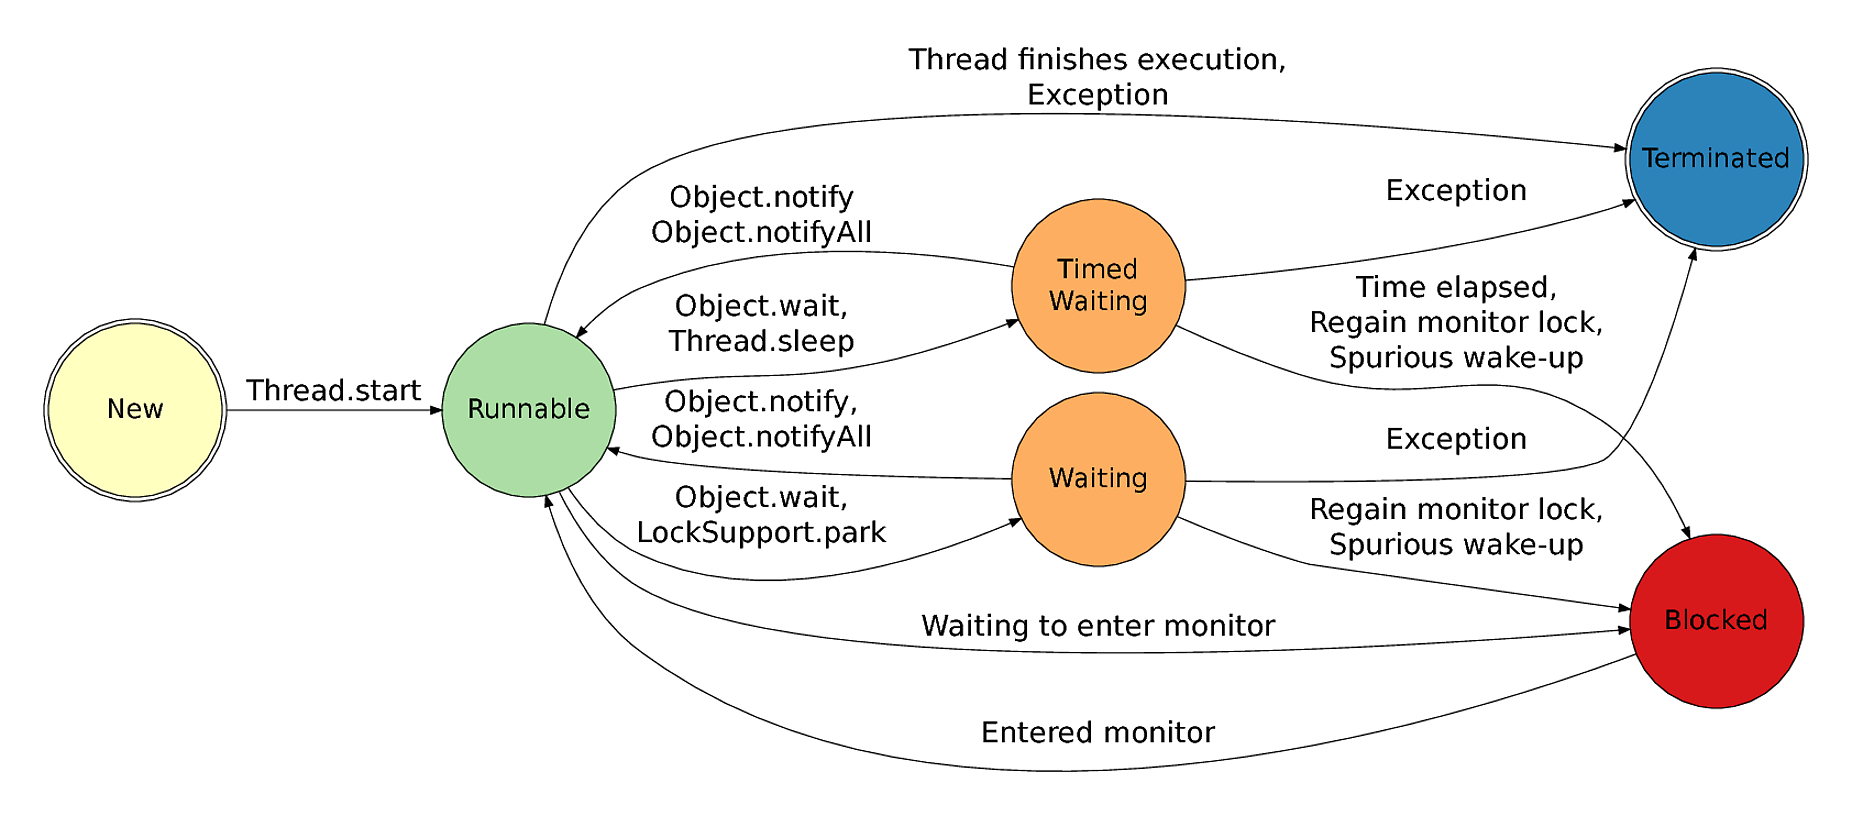
\includegraphics[scale=0.2]{ThreadStateDiagram.png}
    \caption{Java Thread State Diagram. Credit: https://konradreiche.com/}
\end{figure}
\subsubsection{The Timed Waiting State}
This is similar in behaviour to the normal waiting state. Methods that cause a state transition to the timed waiting:
\begin{itemize}
  \item Object.wait(long timeout): This causes the thread to wait on the Object monitor until either the timer elapses or another thread calls notify()/notifyAll() on the monitor.
  \item Thread.sleep(long millis): This method causes the Thread object to pause execution for the specified number of milliseconds. Note that this thread cannot be woken up by any notify(). The method does not have anything to do with monitors, wait() and notify().
  \item Thread.join(long millis): This causes the calling thread to wait for either the timer to expire or the joined thread to terminate (whichever happens first).
\end{itemize}
There are also other methods leading to this transition, but we will not work with them for the remainder of this course. Note that the specified wait times are not guaranteed to be exact, as the underlying OS is responsible for the timing.
\subsubsection{Java Thread States vs OS Thread States}
A question that might come to mind is whether these states are just defined and managed by Java or if they also exist on the OS level. The answer is that in most operating systems, these states also exist. However, Java does not specify how it maps Java thread states to OS thread states. Java leaves this open to the specific JVM implementation. This makes sense, since different JVMs run on different underlying operating systems, which can differ greatly.
\subsubsection{State Transitions in wait()/notify()}
Let us now specifically focus on the thread state transitions occuring in wait()/notify():
\begin{figure}[H]
    \centering
    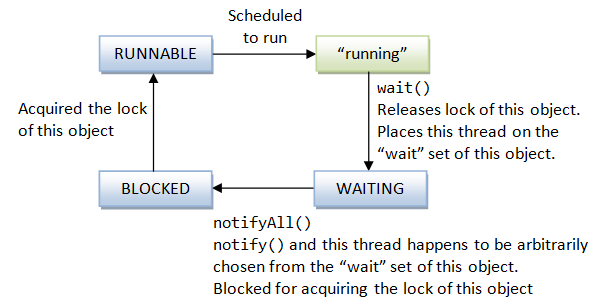
\includegraphics[scale=0.8]{WaitNotifyStates.png}
    \caption{Java Thread State Diagram. Credit: https://konradreiche.com/}
\end{figure}
A running thread (owning a monitor) calling wait() will release the monitor and change to a waiting state. The waiting thread will not continue executing its code until notified by another thread (except for the discussed rare spurious wakeups). Note here that the thread is in a waiting state on the Java language level. It may or may not actually be transitioned to a waiting state on the OS level. The difference is that if it is in a waiting state on the OS level, it will not be scheduled until notified (or spuriously woken up). But Java could also decide to implement the call to wait() as a busy wait, in which case the underlying OS thread is still scheduled (to execute its busy wait instructions). This mapping is not specified in the Java documentation and is implementation dependent.\\
Upon being notified, the thread changes to a blocked state, because before being runnable, the thread needs to reacquire the monitor. This blocked state can be imagined as the waiting area for the monitor.\\
When the monitor is acquired, the thread goes back to a runnable state and once scheduled will continue with the next instruction after the call to wait().

\subsubsection{State Transitions in join()}
What state does a thread transition to when calling Thread.join()? To answer this, let us look at a specific Java implementation of the join() method:
\begin{minted}[]{java}
public final synchronized void join() throws InterruptedException {
    while(isAlive()) {
            wait(0);
    }
}
\end{minted}
Suppose that Thread object t1 calls t2.join(). The following happens now (assuming our system uses OpenJDK):
\begin{enumerate}
  \item The calling thread t1 acquires the monitor of t2.
  \item t1 checks if t2 is not yet terminated.
  \item t1 calls t2.wait(). This transitions t1 to a waiting state.
  \item Upon terminating, t2 notifies on its monitor, causing t1 to return from a waiting state. You may ask where notify() is called. In the OpenJDK implementation, it is called in an internal method when t2 is terminating.
\end{enumerate}
This is the code that is executed when calling join() (without specifying a timeout) in OpenJDK. Note that this is just one specific implementation of Java, and there are others, like the OracleJDK. We are just looking at this code to get an idea of how join() can be implemented, but we cannot assume that every Java implementation executes equivalent code.

% \subsection{Questions That Might Come Up While Reading}
% These are questions that are not directly relevant for the course, but might help understand some concepts better.
% \begin{itemize}
%         \item We talked about thread state diagrams. Are these states managed by the JVM or by the OS itself?
% \end{itemize}

% \subsection{Terminology}
% The most important definitions of this chapter are stated here to be used as a look-up table.
% \begin{itemize}
%   \item \textbf{Deadlock} describes a situation where two or more threads are blocked forever waiting for each other.
%   \item \textbf{Spurious wakeup} occurs when a waiting thread is woken up without being notified. One of the reasons we need to check the condition for a wait() call in a while-loop (instead of an if-statement).
%   \item \textbf{Critical section} is a piece of code that only one thread should be executing at a time (mutual exclusion required).
% \end{itemize}
\end{document}
